\chapter{Aplikace a ukázková hra}
V této části popíšeme instalaci aplikace, použití grafického rozhraní a uvedeme návod pro hraní ukázkové hry. 

\section{Instalace}
Pro instalaci platformy spusťte soubor \texttt{setup.exe}, umístěný v Přílohách práce. Po spuštění instalátoru budete vyzváni k výběru umístění aplikace. Následně bude aplikace nainstalována spolu se všemi svými závislostmi. V aktuální verzi je jedinou závislostí platformy Microsoft .NET Framework 4.7.2 (x86 and x64).

\section{Grafické rozhraní}
Grafické uživatelské rozhraní platformy je tvořeno několika obrazovkami, které můžeme vidět na diagramu \ref{fig:screen_structure2}. Přechody mezi obrazovkami jsou iniciovány za použití grafických prvků těchto obrazovek, či jsou řízeny průběhem akce na pozadí. V této části popíšeme použití složitějších obrazovek uživatelského rozhraní.

\begin{figure}[h]
	\centering
	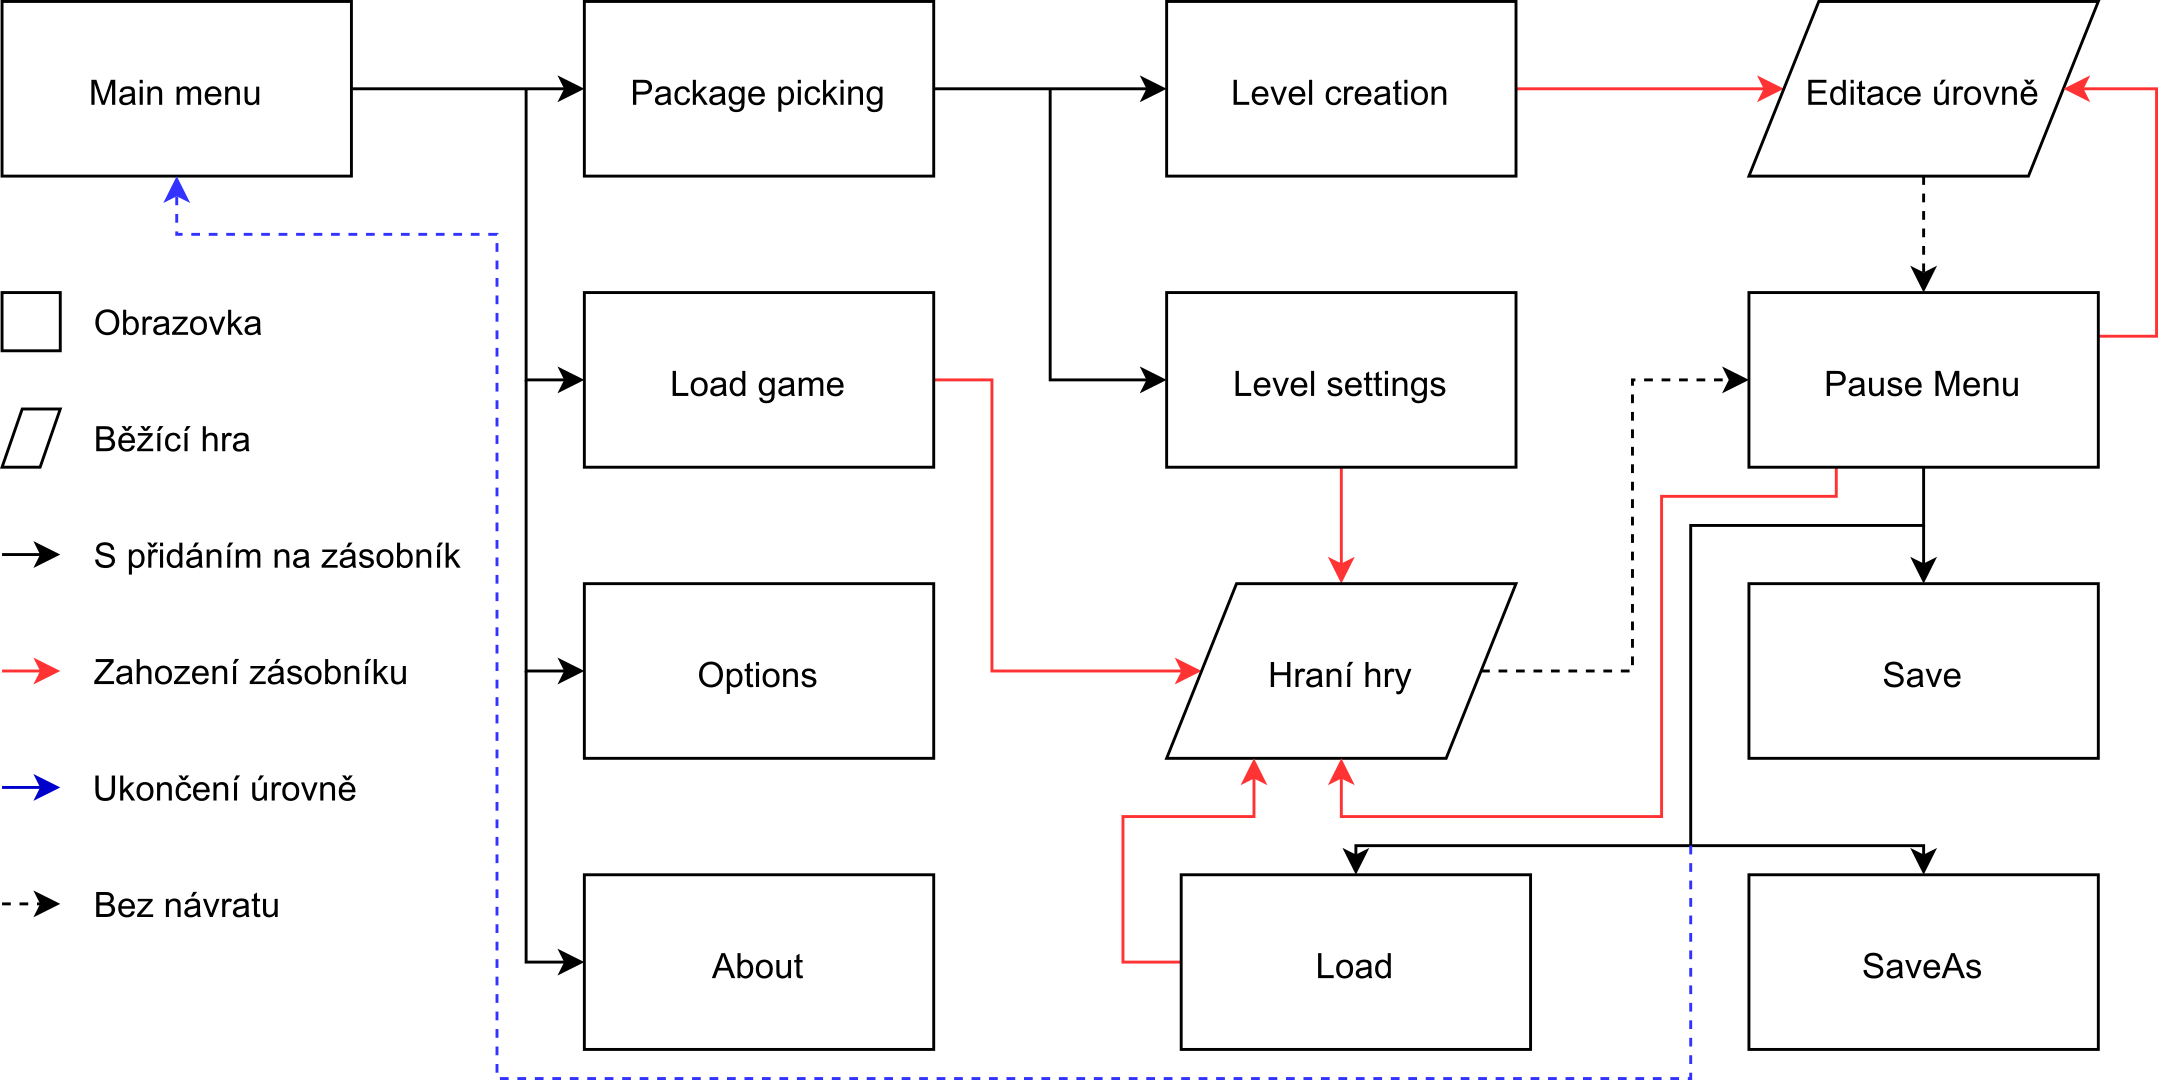
\includegraphics[width=\textwidth]{img/ScreenStructure.png}
	\caption{Obrazovky menu a přechody mezi nimi.}
	\label{fig:screen_structure2}
\end{figure}

\subsection{Výběr balíčků}
Obrazovka pro výběr balíčků, na diagramu \ref{fig:screen_structure2} označena jako \texttt{Package picking}, je z hlavního menu přístupná stisknutím tlačítka \texttt{Start}. Obrazovku můžeme vidět na obrázku \ref{fig:packagepicking}. Centrální část obrazovky zabírá seznam balíčků dostupných v aktuální instalaci platformy. Každý z balíčků je reprezentován jednou položkou tohoto seznamu. 

\begin{figure}[h]
	\centering
	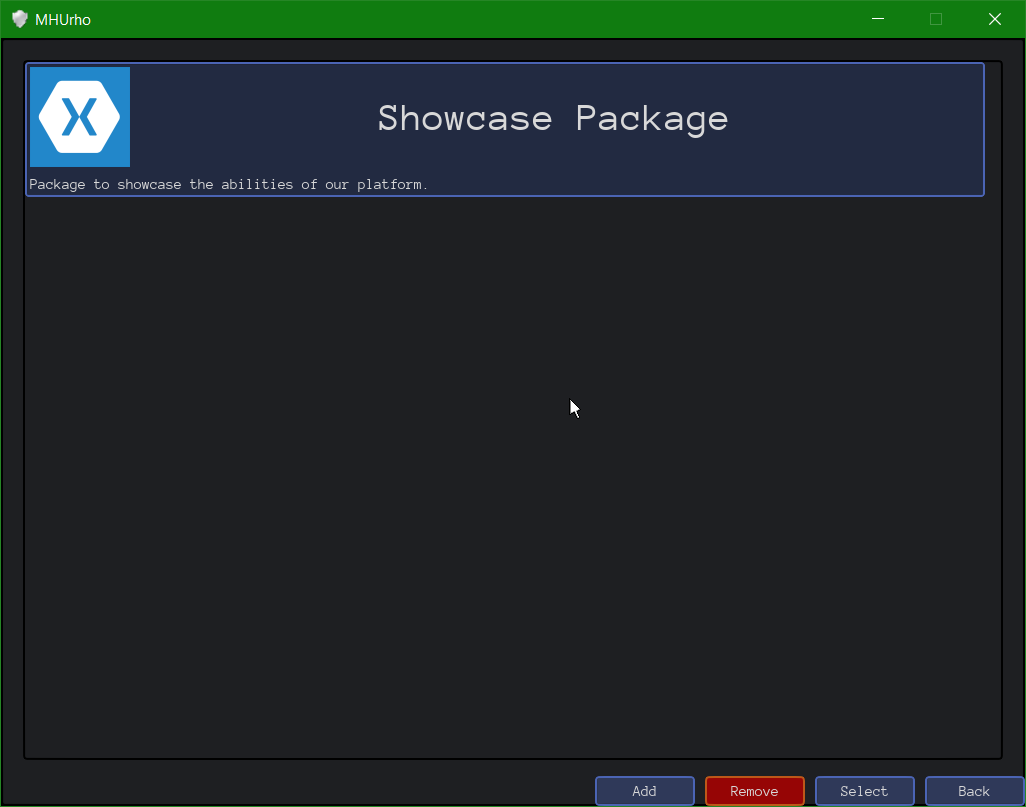
\includegraphics[width=0.5\textwidth]{img/PackagePickingScreen.png}
	\caption{Obrazovky pro výběr balíčku.}
	\label{fig:packagepicking}
\end{figure}

Pro přidání nového balíčků do nainstalované instance platformy přemístěte adresář obsahující soubory balíčku do adresáře \texttt{\%AppData\%/MHUrho/Packages}. Následně stiskněte tlačítko \texttt{Add}, neboli \uv{Přidat}, na obrazovce pro vybírání balíčků. Toto tlačítko vás přesune na obrazovku pro procházení souborového systému. Na této obrazovce poté vyberte XML soubor definující přidávaný balíček. Při návratu na obrazovku pro vybírání balíčků by měl být přidaný balíček viditelný v seznamu dostupných balíčků. d

Pro smazání balíčku označte položku balíčku v seznamu a stiskněte tlačítko \texttt{Remove}. Pro načtení balíčku  označte položku balíčku a stisknute tlačítko \texttt{Select}. Pro návrat na obrazovku hlavního menu použijte tlačítko \texttt{Back}.

\subsection{Výběr úrovně}
Po vybrání balíčku budete přesunuti na obrazovku výběru úrovně, v diagramu označenou jako \texttt{Level picking}. Tuto obrazovku můžete vidět na obrázku \ref{fig:levelpicking}. Tato obrazovka poskytuje následující funkce:

\begin{enumerate}
	\item vytváření a editaci nových úrovní,
	\item editaci existujících úrovní,
	\item spuštění existujících úrovní,
	\item mazání úrovní v balíčku.
\end{enumerate}

Pro vytvoření nové úrovně označte položku \texttt{Create new level} a následně stiskněte tlačítko \texttt{Edit}.

\begin{figure}[h]
	\centering
	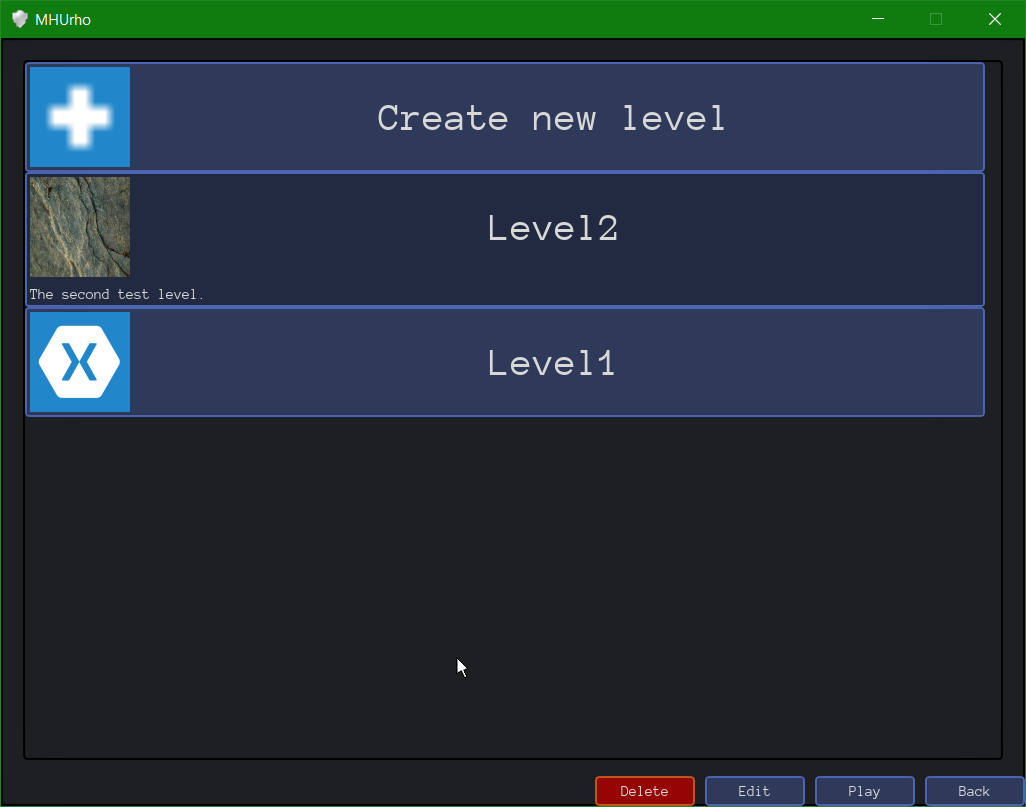
\includegraphics[width=0.5\textwidth]{img/LevelPickingScreen.png}
	\caption{Obrazovky pro výběr úrovně.}
	\label{fig:levelpicking}
\end{figure}

Pro akci s existující úrovní označte tuto úroveň v seznamu. Následně stisknutím tlačítka \texttt{Delete} smažete úroveň, stisknutím tlačítka \texttt{Edit} přejdete na obrazovku \texttt{Level creation} a následně na editaci úrovně a stisknutím tlačítka \texttt{Play} přejdete na obrazovku \texttt{Level settings} pro nastavení parametrů spuštění úrovně.

Pro návrat na obrazovku výběru balíčků použijte tlačítko \texttt{Back}.
\subsection{Vytváření úrovně}
Při vytváření úrovně či editaci existující úrovně budete přesunuti na obrazovku označenou v diagramu \ref{fig:screen_structure2} jako \texttt{Level creation}. Vzhled této obrazovky můžete vidět na obrázku \ref{fig:levelcreation}. Jak můžete vidět, tato obrazovka umožňuje nastavit tyto vlastnosti úrovně:

\begin{enumerate}
	\item jméno,
	\item velikost mapy,
	\item plugin logiky,
	\item ikonu,
	\item popis.
\end{enumerate}

Při editaci existující úrovně nelze měnit její velikost a plugin logiky.

\begin{figure}[h]
	\centering
	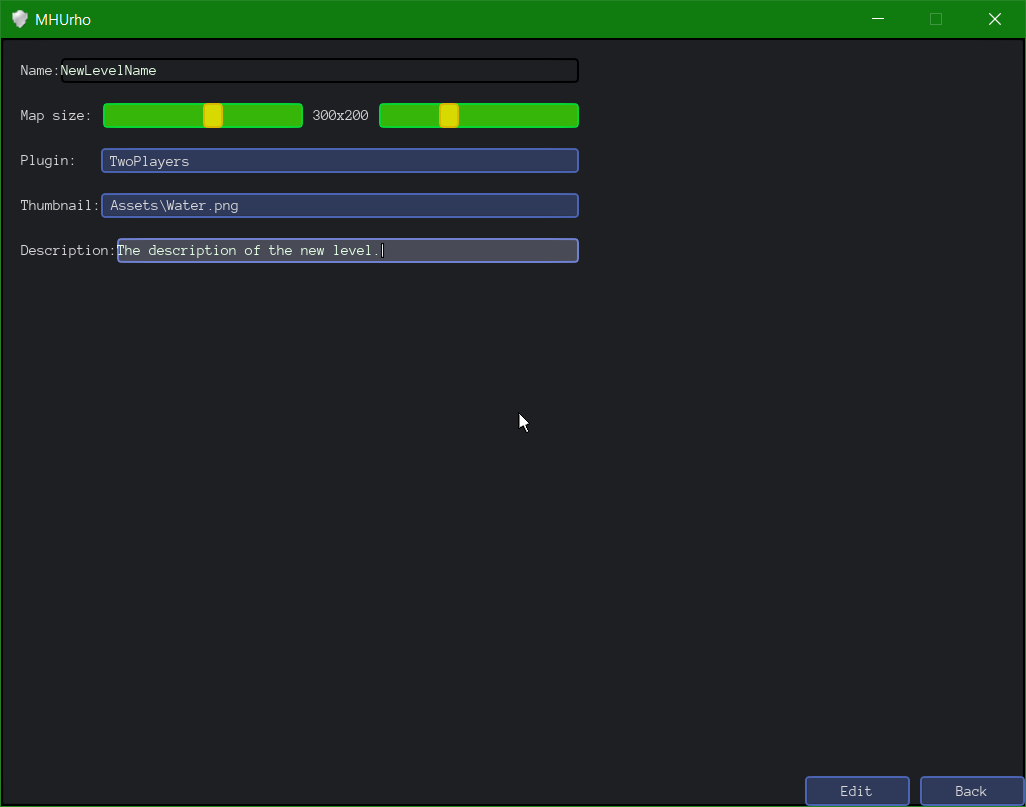
\includegraphics[width=0.5\textwidth]{img/LevelCreationScreen.png}
	\caption{Obrazovky pro nastavení vlastností vytvářené úrovně.}
	\label{fig:levelcreation}
\end{figure}

Pro návrat na obrazovku výběru úrovní použijte tlačítko \texttt{Back}.

\subsection{Nastavení úrovně}
Pro nastavení úrovně před samotným spuštěním slouží obrazovka \texttt{Level settings}, zobrazená na obrázku \ref{fig:levelsettings}. Obrazovka je rozdělena do čtyř částí:

\begin{enumerate}
	\item výběr pluginu hráčů úrovně a nastavení jejich příslušenství do týmu;
	\item zobrazení ikony úrovně;
	\item zobrazení prvků grafického uživatelského rozhraní definovaných pluginem úrovně, používaných pro nastavení parametrů spouštěné úrovně;
	\item zobrazení popisu úrovně.
\end{enumerate}

Stisknutím tlačítka \texttt{Play} je spuštěno načítání úrovně a následně hra. Stisknutím tlačítka \texttt{Back} dojde k přesunu zpět na obrazovku vybírání úrovní.

\begin{figure}[h]
	\centering
	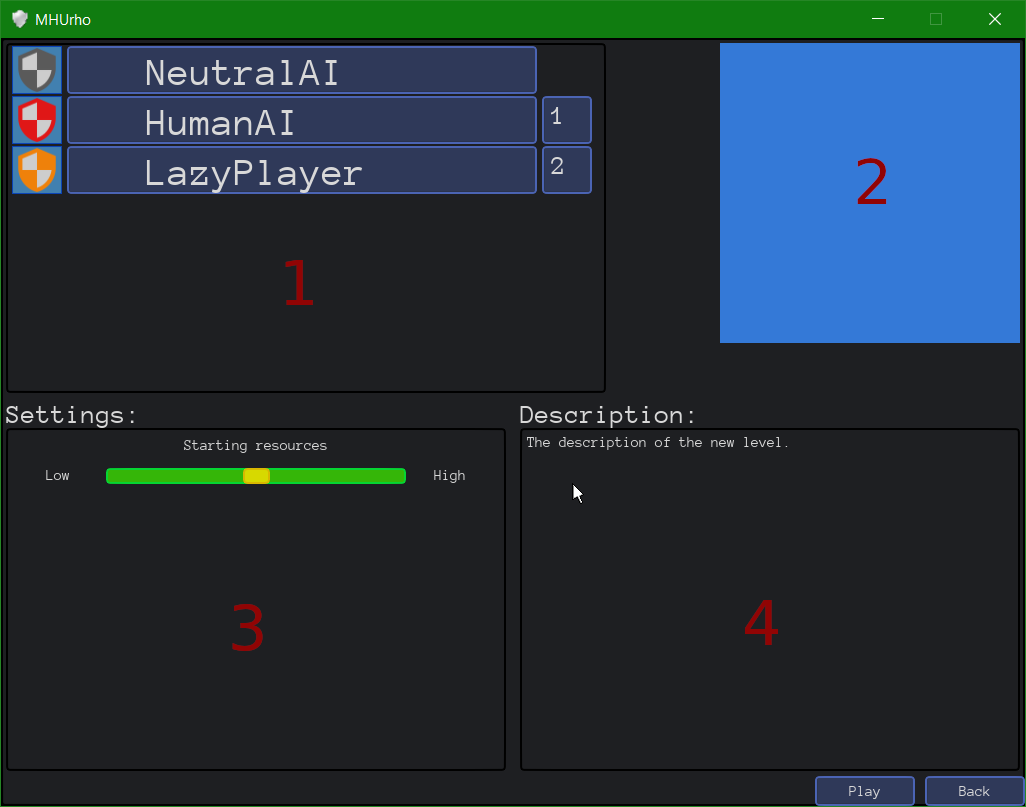
\includegraphics[width=0.5\textwidth]{img/LevelSettingsScreen.png}
	\caption{Obrazovky pro nastavení spuštěné hry.}
	\label{fig:levelsettings}
\end{figure}

\subsection{Přerušení hry}
Při pozastavení hry je zobrazeno tzv.~\texttt{PauseMenu}. Položky tohoto menu se liší podle toho, zda úroveň editujeme či úroveň hrajeme. Porovnání těchto dvou menu můžeme vidět na obrázku \ref{fig:pauseMenu}.

Při editaci umožňuje menu uložit aktuální stav úrovně do balíčkupod jménem nastaveným při vytváření úrovně pomocí tlačítka \texttt{Save} či pod novým jménem pomocí tlačítka \texttt{SaveAs}.

Při hraní hry umožňuje menu uložit aktuální stav hrané hry do adresáře platformy pomocí tlačítka \texttt{Save}, či načíst hranou hru uloženou v tomto adresáři pomocí tlačítka \texttt{Load}.

\begin{figure}[h]
	\centering
	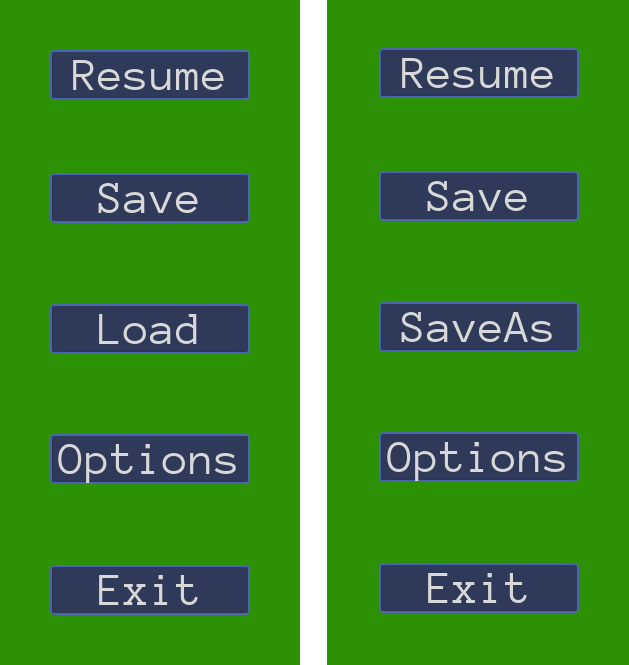
\includegraphics[width=0.5\textwidth]{img/PauseMenuComparison.png}
	\caption{Menu pozastavení hry.}
	\label{fig:pauseMenu}
\end{figure}


\subsection{Výběr souboru}
Obrazovku pro výběr souboru můžeme vidět na obrázku \ref{fig:filepicking}. Modře označená část výpisu obsahu adresáře představuje podadresáře, bílá část pak soubory. V horní části můžeme vidět vyhledávací řádek, do kterého je možno napsat část jména pro filtrování zobrazených souborů či přímo celou cestu vybíraného souboru či adresáře. Pro výběr lze použít tlačítko \texttt{Select}, které vybere soubor či adresář podle cesty ve vyhledávacím řádku, či dvojklikem na záznam vybíraného souboru.

Obrazovky pro ukládání a načítání hraných úrovní z adresáře platformy poskytují navíc tlačítko \texttt{Delete}, kterým je možné úložku smazat.

\begin{figure}[h]
	\centering
	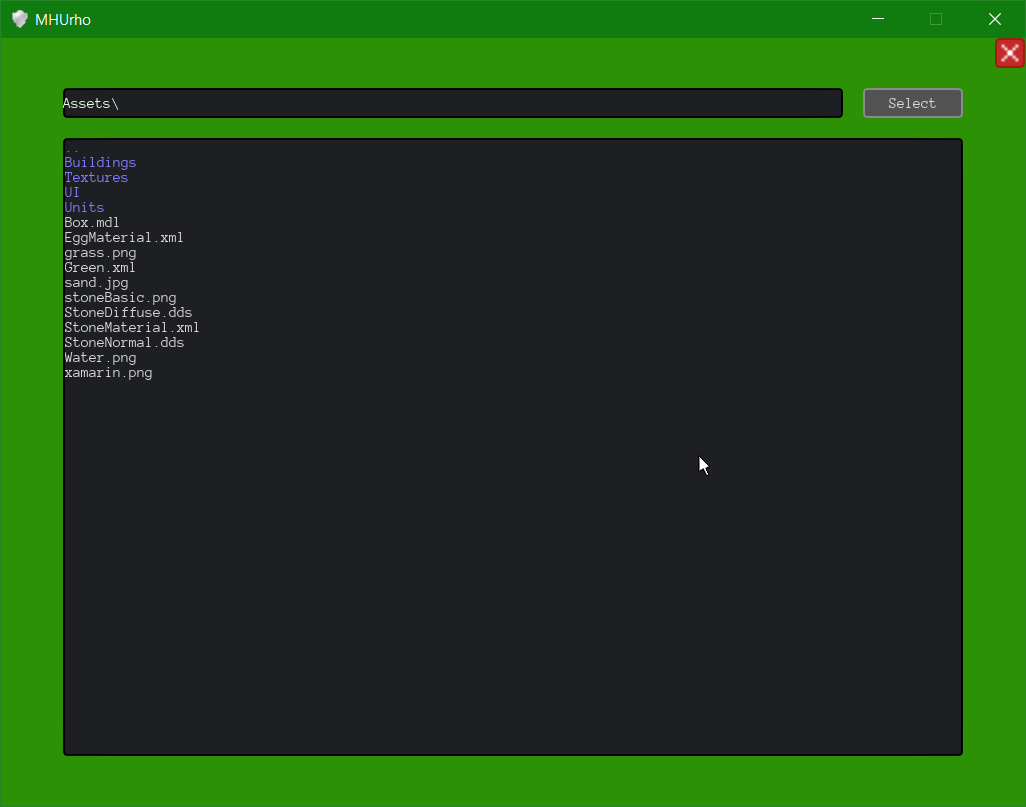
\includegraphics[width=0.5\textwidth]{img/FilePickingScreen.png}
	\caption{Obrazovka pro výběr souboru.}
	\label{fig:filepicking}
\end{figure}

\section{Ukázková hra}
Ukázková hra je reprezentována balíčkem \texttt{ShowcasePackage}. Tento balíček obsahuje jednotky, budovy, projektily a další součásti hry, které je možné využít pro tvorbu úrovní. Současně obsahuje několik již vytvořených úrovní demonstrujících schopnosti protihráčů, jednotek a budov.

\subsection{Okno aplikace při hře}
\label{sec:appwindow}
Okno aplikace má při hře platformou definované základní uživatelské rozhraní. Toto rozhraní můžeme vidět na obrázku \ref{fig:UI}. 

Minimapa poskytuje hráči přehled o stavu velké části mapy bez nutnosti pohybu kamerou. Minimapu lze přibližovat či oddalovat za použití kolečka myši při umístění kurzoru nad minimapu. Dále lze kliknutím přesunout kameru na odpovídající pozici v herním světě. V neposlední řadě lze minimapu použít k rychlému přesunu kamery pomocí kliknutí a držení levého tlačítka a posunu myší. Pozice kliknutí se stává středem pomyslného joysticku, který ovládáme posunem myši odpovídajícím směrem.

Centrální lišta obsahuje tlačítka určená aktuálně zvoleným nástrojem. Při velkém počtu tlačítek je možno touto lištou posouvat za použití tlačítek označených šipkami na pravé a levé straně lišty.

Nad lištou vidíme vpravo tlačítko pro výběr aktuálního hráče a vlevo tlačítko pro výběr nástroje. Výběr hráče je možný pouze při editaci úrovně. Při hraní je toto tlačítko neaktivní a pouze zobrazuje ikonu hráče reprezentujícího uživatele. Tlačítko pro výběr budovy, stejně jako tlačítko pro výběr hráče při editaci, při kliknutí zobrazí vysouvací lištu, označenou fialově. Tato lišta obsahuje seznam dostupných nástrojů či seznam dostupných hráčů.

Poslední součástí v levém dolním rohu je \texttt{CustomWindow}. Obsah této části je určen aktuálním nástrojem. Nejčastěji je v této části uváděn název nástroje či součásti nástroje, nastavní velikosti štětce, cena budov a další.

Balíček může do uživatelského rozhraní dodat vlastní prvky, jak můžeme vidět ve vrchní části obrazovky, ve které balíček ukázkové hry umisťuje lištu pro zobrazení množství surovin vlastněných hráčem.

\begin{figure}[h]
	\centering
	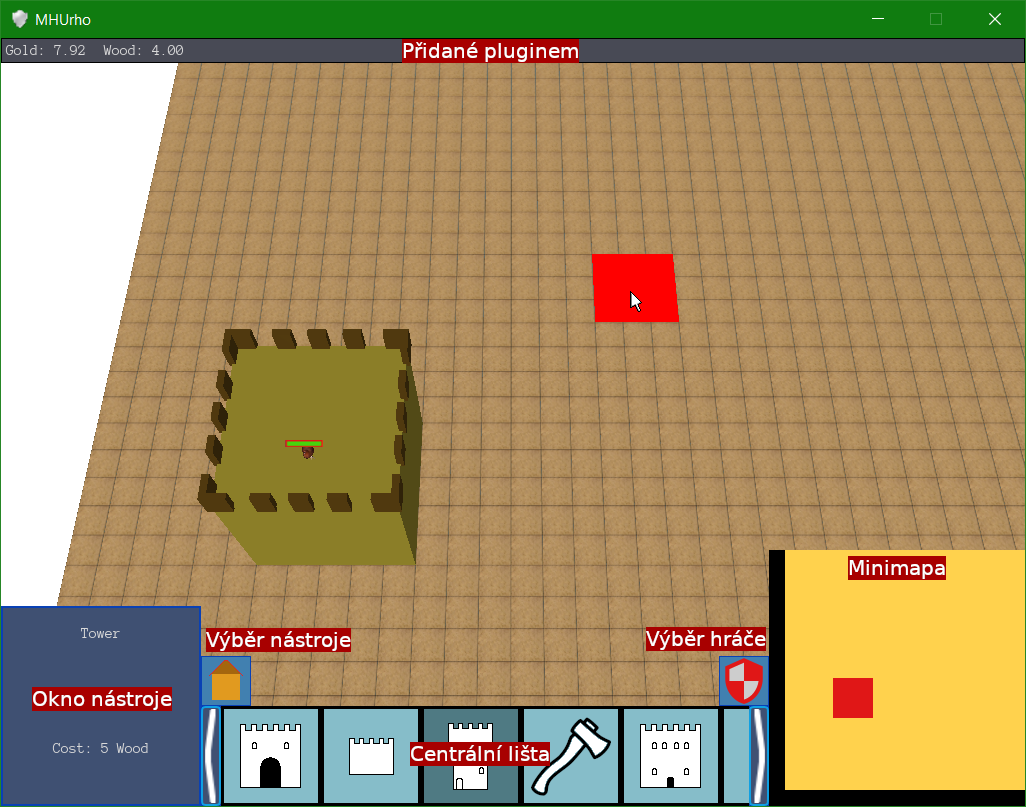
\includegraphics[width=0.5\textwidth]{img/GameUI.png}
	\caption{Uživatelské rozhraní ukázkové hry.}
	\label{fig:UI}
\end{figure}

\subsection{Editor}
Každý z balíčků, tedy i ukázková hra, může definovat své vlastní nástroje pro editaci úrovně, či použít nástroje poskytované platformou. V této části popíšeme použití nástrojů dostupných v editoru úrovní ukázkové hry.

\subsubsection{Editace terénu}
Editace terénu je umožněna dvěma nástroji, a to \texttt{TerrainManipulator}, tedy manipulátor terénu, a \texttt{TileTypeTool}, tedy nástroj pro změny typů dlaždic. 

Nástroj \texttt{TerrainManipulator} umožňuje tyto změny terénu:

\begin{enumerate}
	\item nástroj pro výběr rohů dlaždic,
	\item nástroj pro změnu výšky vybraných rohů dlaždic,
	\item nástroj pro změnu výšky skupiny dlaždic
	\item nástroj pro vyhlazení terénu.
\end{enumerate}

Nástroj pro změny typů dlaždic naplní centrální lištu tlačítky všech typů dlaždic v balíčku. Po vybrání jednoho z typů je pak možné kliknutím na část mapy změnit tuto typ dlaždic v této části. Velikost měněné částí lze nastavit v okně nástroje.

\subsubsection{Stavba budov}
Nástroj pro stavbu budov je jeden ze dvou nástrojů dostupných v módu editace úrovně i v módu hry. Centrální lišta je naplněna tlačítky pro všechny typy budov dostupných pro stavbu v aktuálním módu. Množiny se v ukázkové hře liší mezi editačním a hraným módem.

V herním módu tento nástroj umožňuje při kliknutí bez zvolené budovy zobrazit uživatelské rozhraní budov brány i tvrze a tím nám umožňuje jejich ovládání.

\subsubsection{Tvorba jednotek}
Nástroj pro tvorbu jednotek umožňuje umisťovat do herního světa nové jednotky, případně mazat existující jednotky. Lišta tohoto nástroje obsahuje seznam jednotek, které je možno manuálně přidávat do herního světa. Poslední tlačítko, obsahující červený čtverec, reprezentuje nástroj pro mazání existujících jednotek.

Funkcionalita tohoto nástroje je při hraní úrovně nahrazena budovou tvrze, popsanou v části \ref{sec:defbuildings}.

\subsubsection{Ovládání jednotek}
Nástroj pro ovládání jednotek umožňuje označení skupiny jednotek a následné vydávání rozkazů této skupině. Pomocí tohoto nástroje lze jednotkám vydat rozkaz na přemístění na pozici v mapě či na útok na nepřátelskou jednotku.


\subsection{Ovládání kamery}
Kamera je schopna pohybu v několika módech. Těmito módy jsou RTS mód, \texttt{FreeFloat} mód a sledování jednotky. Přepínání mezi RTS a \texttt{FreeFloat} módem je prováděno klávesou \textit{Shift}. Přepnutí na sledování jednotky je možné kliknutím pravého tlačítka na jednotku. Následná lze přejít zpět na RTS mód pokusem o pohnutí kamerou, či na \texttt{FreeFloat} mód pomocí klávesy \textit{Shift}.

Pohyb v módech RTS a \texttt{FreeFloat} lze ovládat pomocí klávesnice. Klávesy \textit{W}, \textit{S}, \textit{A}, \textit{D} umožňují pohyb kamery vpřed, vzad, vlevo a vpravo. 

V módu RTS lze také ovládat pohyb kamery pomocí umístění myší na okraj obrazovky, načež se kamera začne posouvat směrem k tomuto okraji. 

Otáčení kamery lze v RTS módu a módu sledování jednotky provést klávesami \textit{Q} a \texttt{E} pro otáčení vlevo či vpravo, a klávesami \textit{R} a \textit{F} pro otáčení vzhůru a dolu. 

V módu \texttt{FreeFloat} lze otáčet kamerou pouze pomocí myši.   

\subsection{Budovy}
Na diagramu \ref{fig:buildings} vidíme budovy poskytované balíčkem ukázkové hry. Nyní popíšeme jednotlivé typy budov.

\begin{figure}[h]
	\centering
	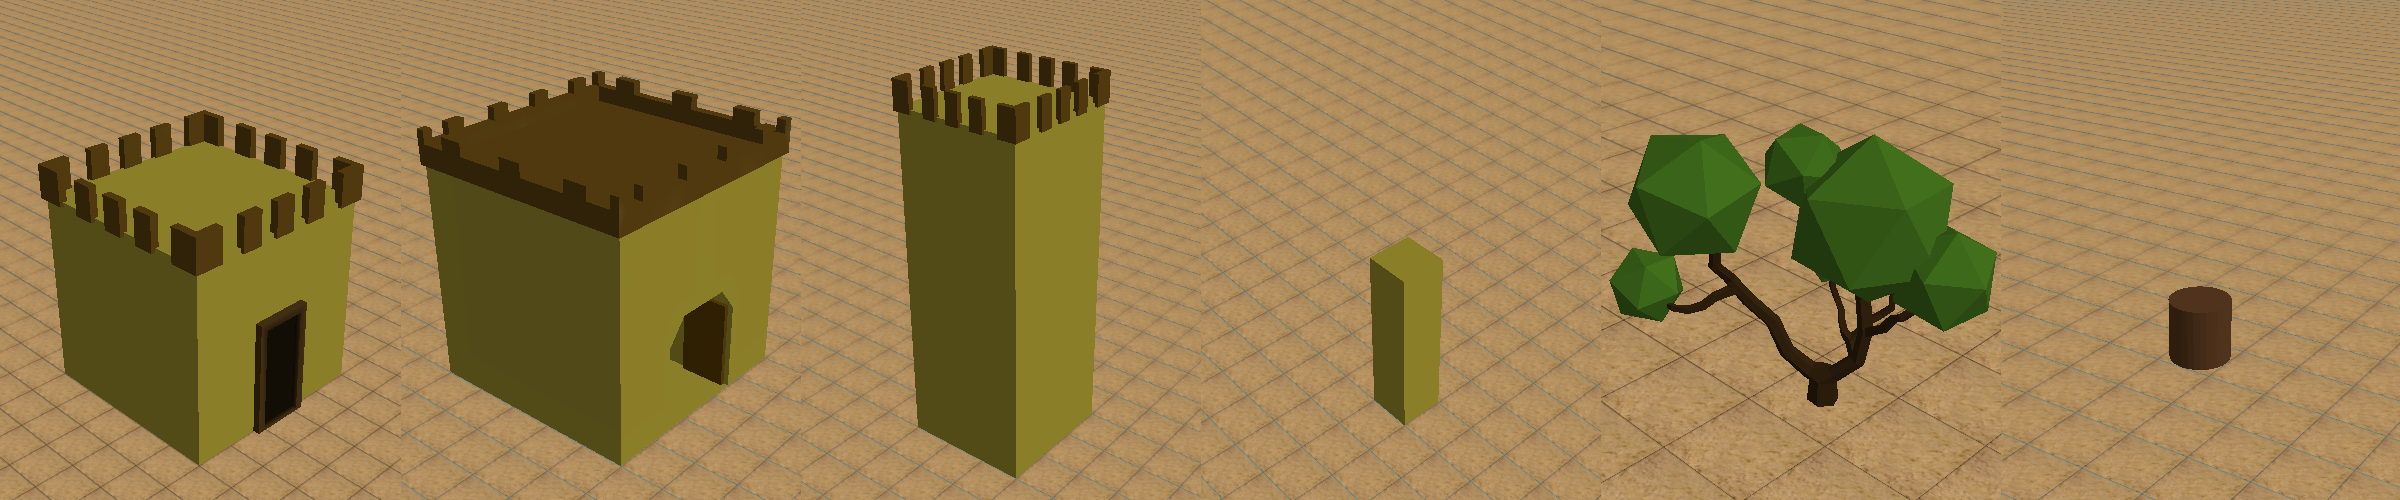
\includegraphics[width=\textwidth]{img/Buildings.png}
	\caption{Budovy v ukázkové hře.}
	\label{fig:buildings}
\end{figure}

\subsubsection{Obranné budovy}
\label{sec:defbuildings}
Prvních čtyři budovy na obrázku \ref{fig:buildings} označujeme jako obranné budovy, sloužící především pro zamezení průchodu nepřátelských jednotek a umožňující zvýšení dostřelu vlastních jednotek pomocí umístění jednotek na tyto budovy.

První budovu je \texttt{Keep}, neboli tvrz. Každý hráč vlastní právě jednu tuto budovu, při jejímž zničení hráč prohrává. Cílem hry je tedy zničit protivníkovu tvrz bez ztráty své vlastní tvrze. Tvrz umožňuje pohyb jednotek po své střeše s možností napojení na střechy ostatních budov umožňujících tuto funkci. Tvrz dále slouží pro tvorbu jednotek během hry. Tato funkce je zpřístupněna pomocí nástroje pro stavbu budov, který kliknutím na tvrz bez vybrané budovy umožňuje zobrazení uživatelského rozhraní.

Druhou budovou je \texttt{Gate}, neboli brána. Brána umožňuje pohyb jednotek jak po své střeše, tak skrz tunel uvnitř této budovy. Dále umožňuje brána již podle svého názvu zavřít jeden konec tunelu a tím znemožnit přístup do tunelu z této strany. Ovládání brány je zpřístupněno pomocí nástroje pro stavbu budov, stejně jako ovládání tvrze. Uživatelské rozhraní pak umožňuje otevírání a zavírání brány.

Třetí budovou je \texttt{Tower}, neboli věž. Tato budova umožňuje chůzi po své střeše a díky své výšce zvyšuje dostřel jednotek.

Čtvrtou budovou je \texttt{Wall}, neboli hradba. Hlavním účelem této budovy je zablokování přístupu do hradu. Dále umožňuje hradba chůzi po své horní části.

\subsubsection{Ostatní budovy}
Zbylé dvě budovy slouží pro získávání dřeva. Těmito budovami jsou \texttt{Tree}, neboli strom, a \texttt{TreeCutter}, neboli dřevorubec.

Stavba stromů je omezena na editaci úrovně a jejich vlastníkem může být pouze neutrální hráče, tedy hráče s šedým štítem. Tento hráč jako jediný nemá tvrz, nelze ho zabít a neútočí na ostatní hráče. Stromy podle typu dlaždice, na které se nacházejí, rostou různou rychlostí a množí se s různou pravděpodobností.

Dřevorubec umožňuje hráči získávat ze stromů dřevo. Tato budova vytváří dvě jednotky, které následně pendlují mezi nejbližším stromem a touto budovou, čímž získávají pro hráče dřevo.

\subsection{Jednotky}
Balíček ukázkové hry definuje dvě jednotky, a to \texttt{Chicken} a \texttt{Wolf}, neboli kuřata a vlky. Vzhled těchto jednotek můžeme vidět na obrázku \ref{fig:units}

\begin{figure}[h]
	\centering
	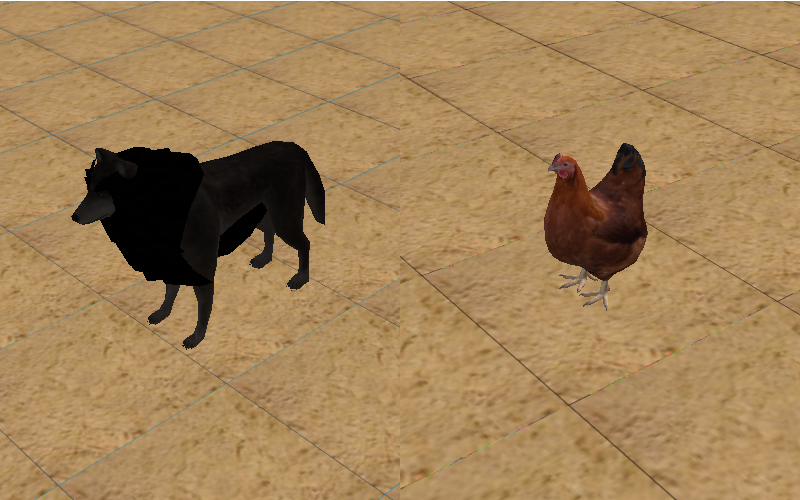
\includegraphics[width=0.5\textwidth]{img/Units.png}
	\caption{Jednotky v ukázkové hře.}
	\label{fig:units}
\end{figure}

\texttt{Chicken} je jednotka útočící na dálku, používající vajíčka jako projektily. Dostřel této jednotky závisí na rozdílu její výšky od cíle, je tedy výhodné ji umisťovat na vyvýšená místa, jako například budovy. Oproti vlkům dokáže tento typ jednotek chodit přes vodu a poškodit obranné budovy.

\texttt{Wolf}, neboli vlk, je jednotka útočící na blízko. Tato jednotka se pohybuje rychleji než \texttt{Chicken} nebo obslužná jednotka budovy dřevorubce. Tato jednotka nedokáže poškodit nepřátelské obranné budovy.


\subsection{Projektily}
Ukázková hra definuje pouze jeden projektilů, ze kterých je pouze jeden aktuálně využíván. Těmito typy jsou:

\begin{enumerate}
	\item \texttt{EggProjectile},
	\item \texttt{TestProjectile}.
\end{enumerate}

První typ je využíván jednotkou \texttt{Chicken}. Tento typ má jednoduchou logiku využívající komponenty \texttt{BallisticProjectile} pro implementaci svého pohybu. Drhý typ ukazuje možnosti složitějšího chování projektilu. Tento projektil také využívá pro implementaci svého pohybu komponentu \texttt{BallisticProjectile}, ale dále přidává dodatečné chování. Po určité době od výstřelu se tento projektil rozdělí na více projektilů stejného druhu, čímž vytvoří efekt brokovnice a pokryje projektily okolí svého původního dopadu. Dále tento projektil ukazuje zpožděné odstranění z úrovně, díky kterému zůstává určitou chvíli zaseknutý v terénu.

\subsection{Umělé inteligence hráčů}
Ukázková hra poskytuje dvě umělé inteligence nepřátelských hráčů, kterými jsou:

\begin{enumerate}
	\item \texttt{LazyPlayer},
	\item \texttt{AggressivePlayer}.
\end{enumerate}

Lazy player je jednoduchá umělá inteligence, která nic nedělá. Jejím hlavním účelem umožnění uživately vyzkoušení herního režimu platformy a možnost stavby svého hradu bez jakéhokoli ohrožení nepřítelem.

AggressivePlayer je aktivní umělá inteligence, která staví budovy pro získávání dřeva, jednotky pro obranu svého tvrze a útok na nejbližšího nepřátelského hráče.

\subsection{Umělé inteligence úrovní}
Ukázková hra je příkladem balíčku, který všechnu svou logiku decentralizuje do jednotek, budov, projektilů a hráčů. Z tohoto důvodu obsahují dvě logiky definované ukázkovou hrou minimum herní logiky. Ukázková hra poskytuje tyto dvě logiky:

\begin{enumerate}
	\item \texttt{TwoPlayerLogic},
	\item \texttt{FourPlayerLogic}.
\end{enumerate}

Obě tyto logiky poskytují požadované metody informace platformě ve formě \texttt{ToolManageru} a \texttt{AStarFactory}. 

První logika již podle názvu definuje úrovně se dvěma hráči. Dále poskytuje možnost před prvním spuštěním úrovně nastavit počáteční množství surovin vlastněné hráči.
Druhá logiky definuje úrovně se čtyřmi hráči a určuje pevné množství počátečních surovin.
